%%中山大学物理学院-基础物理实验-完整实验报告模板1.2
%%完成整理日期:2020/2/18
%%更新时间:2021/1/22
%%中山大学物理学院18级 王佛泓
%%平台:win10, Texlive 2019
%%编译方式:xelatex


%---------------------导言区---------------------------%
\documentclass[12pt,a4paper,UTF8]{ctexart}
	%10pt:正文字体为12pt,缺省为10pt;各层级字体大小会根据正文字体自动调整
	%a4paper:纸张大小a4;
	%UTF8:中文要求
\usepackage{geometry}%用于设置上下左右页边距
	\geometry{left=2.5cm,right=2.5cm,top=3.2cm,bottom=2.8cm}
\usepackage{xeCJK,amsmath,paralist,enumerate,booktabs,multirow,graphicx,subfig,setspace,listings,lastpage,hyperref}
	%xeCJK:中文字体(如楷体,作者和机构需要用到)的设置
	%amsmath:数学公式
	%paralist,enumerate:自定义项目符号
	%booktabs:三线图,论文常用的表格风格
	%multirow:复杂表格
	%graphicx,float: 插入图片
	%subfig:并排排版图片、竖向排版图片
	%setspace:设置行间距等功能
	\setlength{\parindent}{2em}%正文首行缩进两个汉字
	%listings:用于排版各种代码;比如matlab的代码
	\lstset{language=Matlab}%matlab代码
	%lastpage:获取总页数;
	%hyperref:超链接,和lastpage搭配.
\usepackage{fancyhdr}
	%fancyhdr:一个很强大的宏包,用于自定义设计页面风格并命名以供调用。
	\pagestyle{fancy}
	\rhead{实验B12 温度测控仪的设计和组装}
	\lhead{基础物理实验\uppercase\expandafter{\romannumeral2}实验报告}
	\cfoot{Page \thepage/\pageref{LastPage}}  %当前页\总页数
	\rfoot{\today}
		%分别是右页眉、左页眉、中页脚、右页脚
	\renewcommand{\headrulewidth}{0.4pt}
	\renewcommand{\theenumi}{(\arabic{enumi})}

% \setCJKmainfont{FZShuSong-Z01S}[ItalicFont=FZKai-Z03S, BoldFont=FZHei-B01S]
%中文字体设置:使用开源字体方正书宋,方正楷体和方正黑体



%%%%%%%%%%%%%%%%%%%%%%%%%%%%%%%%%%%%%%%%%%%%%%%%%%%%%%%%%%
%%%%%%%%%%%%%%%%%%%%%%%%%正文开始%%%%%%%%%%%%%%%%%%%%%%%%%%
%%%%%%%%%%%%%%%%%%%%%%%%%%%%%%%%%%%%%%%%%%%%%%%%%%%%%%%%%%

\begin{document}

%%begin-------------------标题与信息-----------------------%%

%%标题
\begin{center}
\LARGE\textbf{实验B12温度测控仪的设计和组装}
\end{center}


%%end-------------------标题与信息-----------------------%%


\subsection*{【数据处理与分析】}
\subsubsection*{1.数字电压读数与温度关系}

\begin{figure}[htbp]
	\centering
	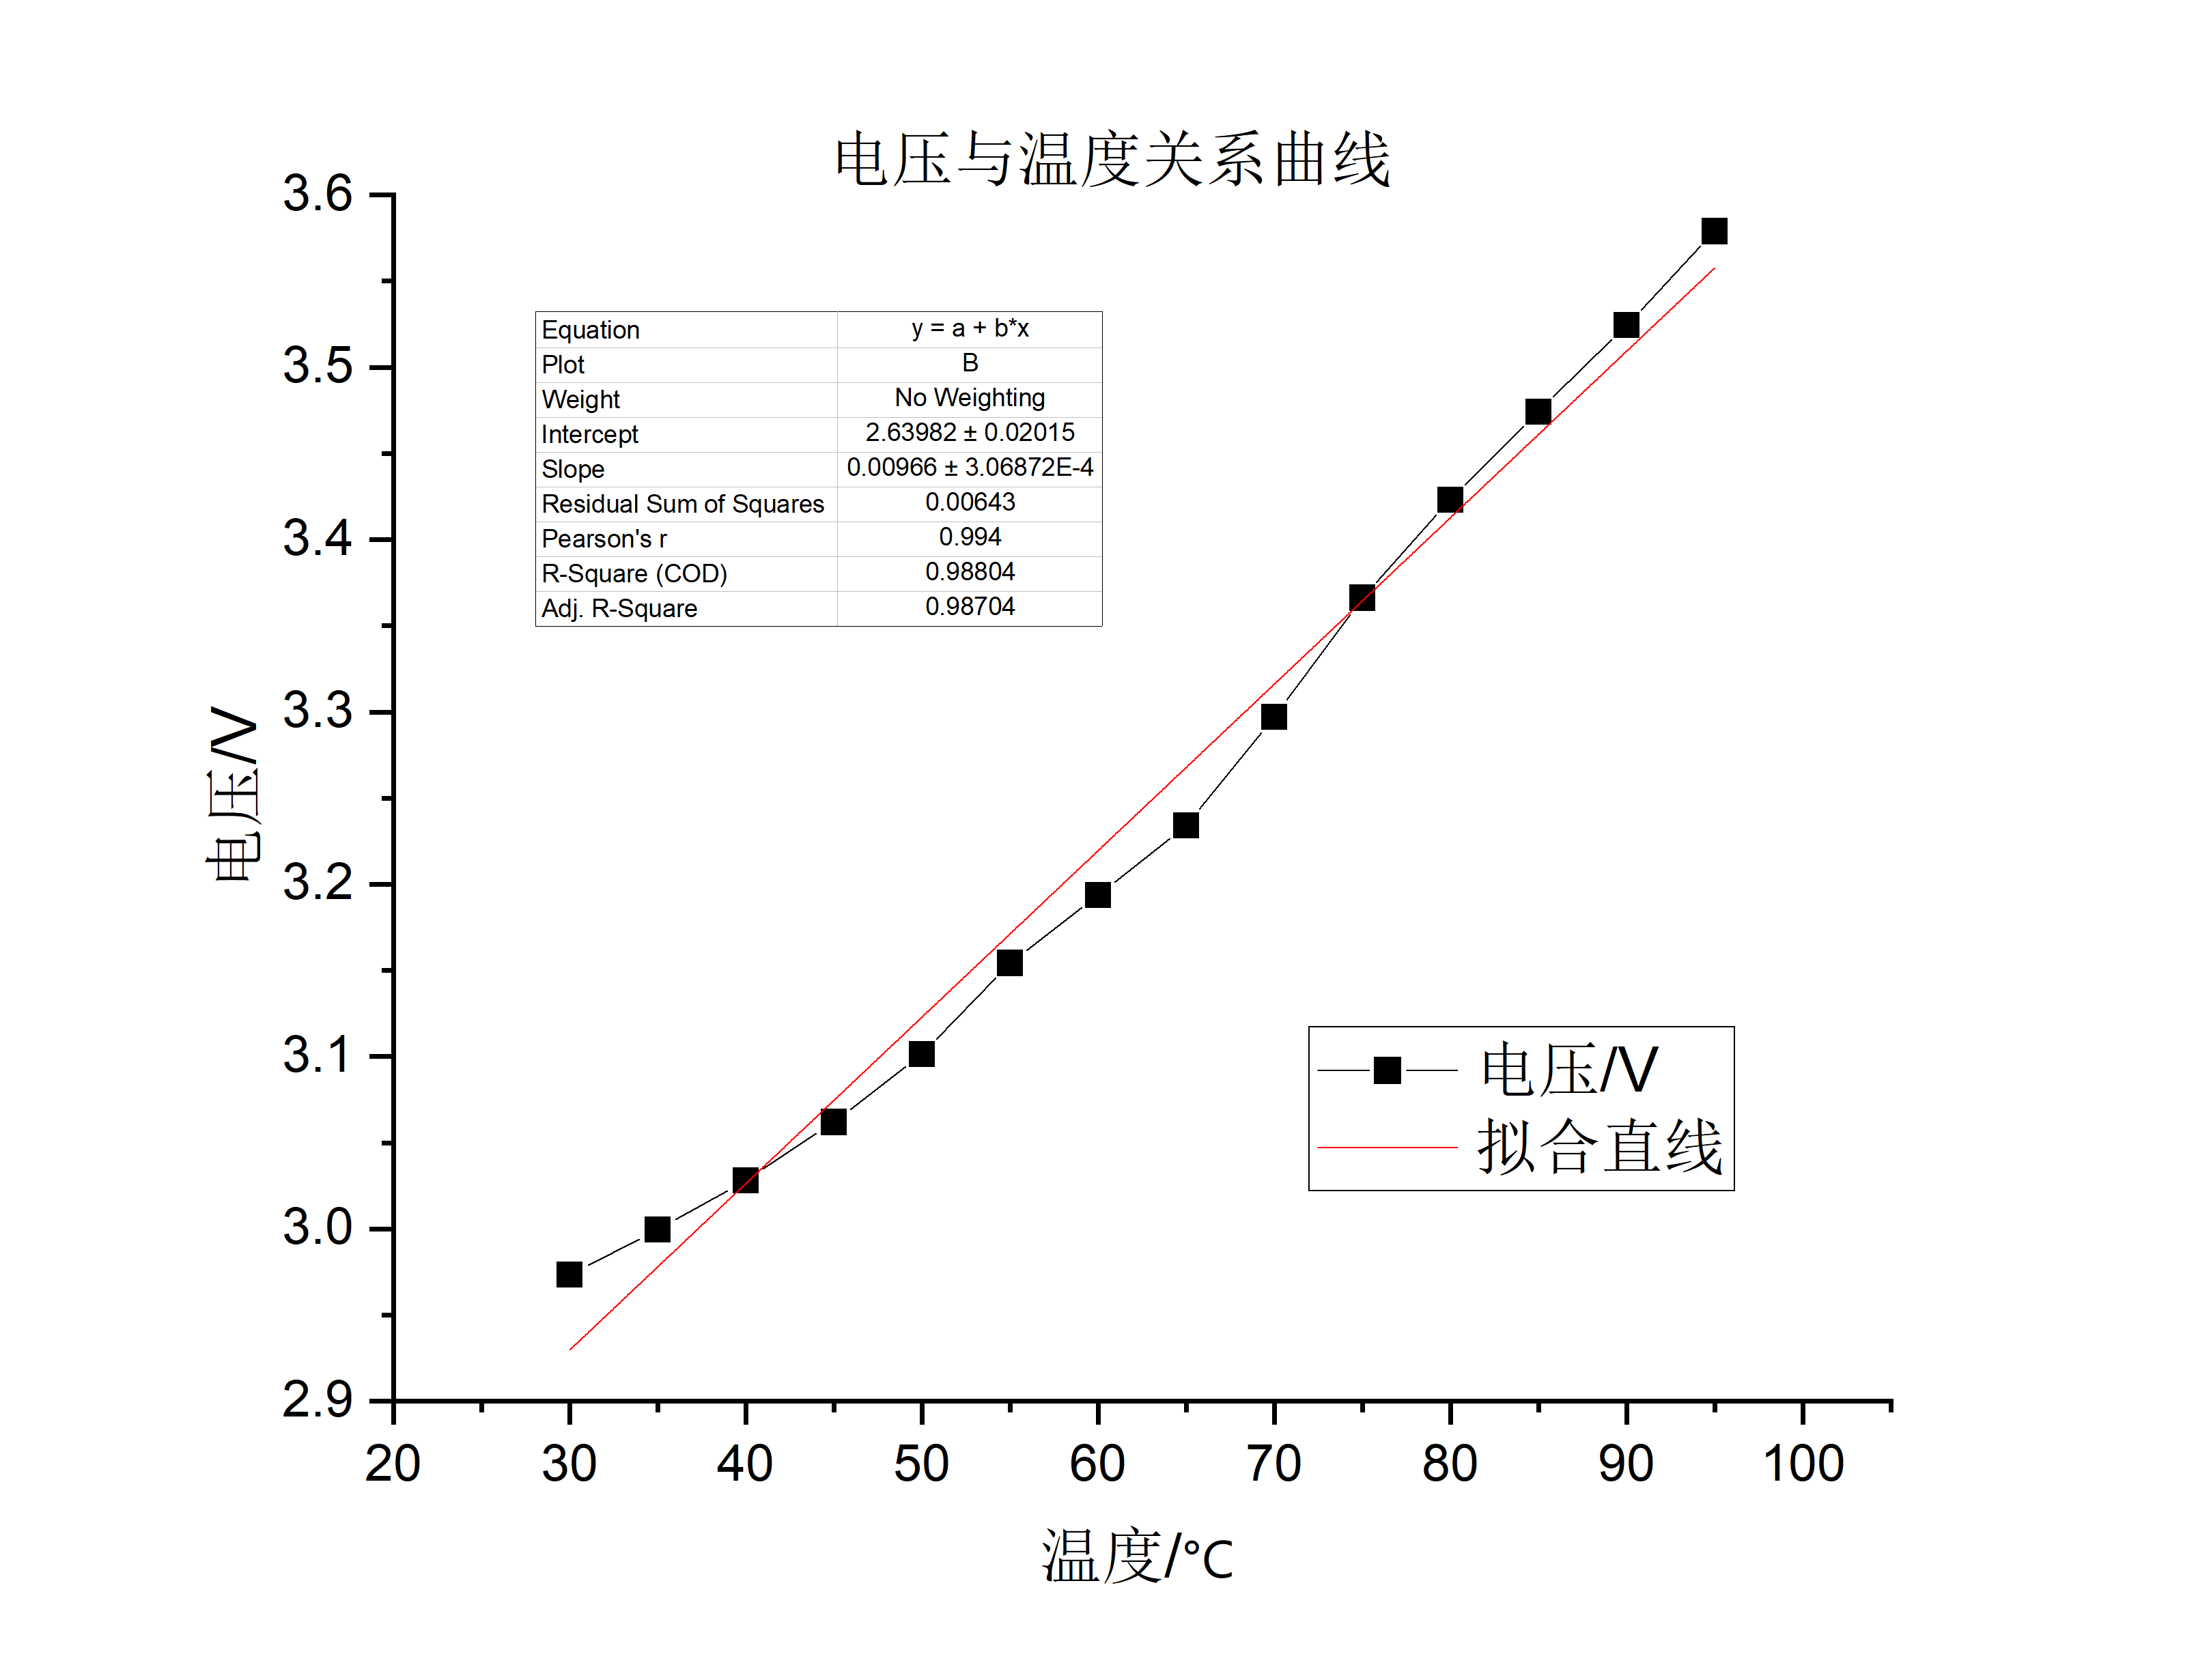
\includegraphics[width=0.8\textwidth]{img//reg.png}
	\caption{电压与温度线性拟合作图}
\end{figure}
线性拟合结果可得电压与温度较好地符合线性关系,每升温一摄氏度,电压增高0.00966V.

存在误差的可能原因有:
\begin{enumerate}
	\item 电压读数误差
	\item 测控仪系统误差
	\item 温度传递需要时间,AD590温度可能与加热阱温度略有差异
\end{enumerate}

\subsubsection*{2.温度测控仪工作过程}

控制温度:
\begin{equation*}
	t= \frac{76.6+71.4}{2}  = 74^{\circ}C
\end{equation*}
相对误差:
\begin{equation*}
	E=\left\lvert \frac{75-74}{74}\right\rvert \times 100\%=1.33\%
\end{equation*}
误差较小。
\begin{figure}[!h]
	\centering
	\subfloat[由亮到暗]{\label{fig:3}
	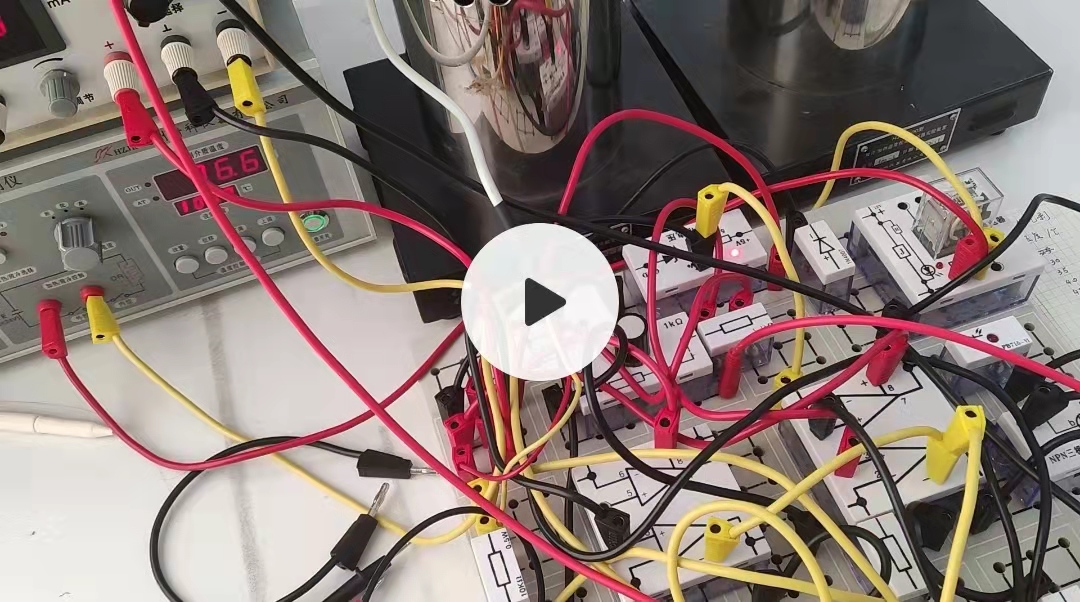
\includegraphics[width=0.4\textwidth]{img/3.jpg}%调节这里的图片宽度
	}%
	\subfloat[由暗到亮]{\label{fig:4}
	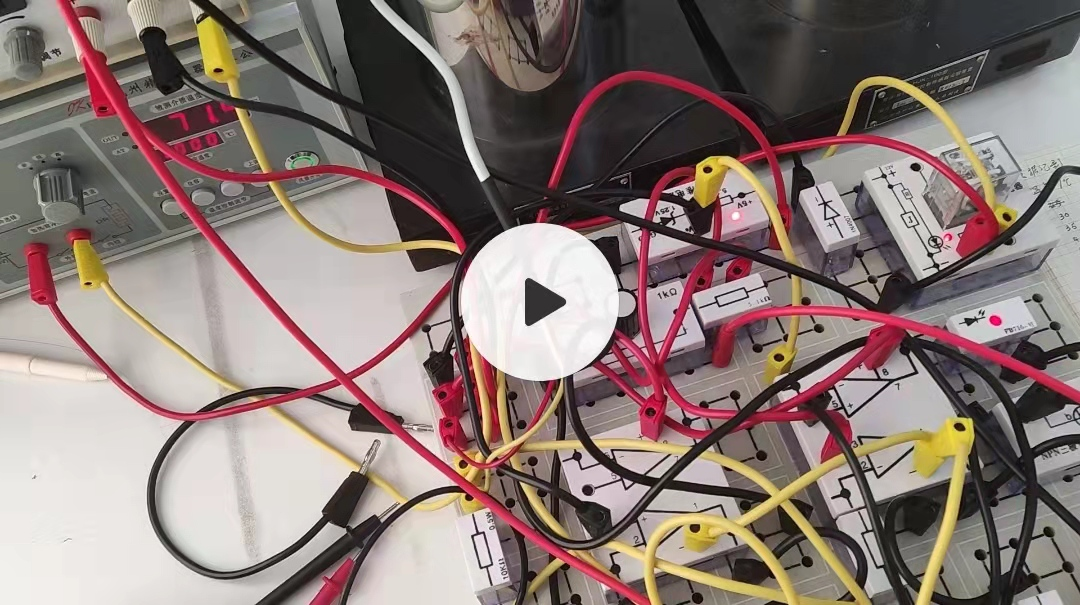
\includegraphics[width=0.4\textwidth]{img/4.jpg}%调节这里的图片宽度
	}%
	\caption{实验过程图片}
	\label{fig:tcvi}
\end{figure}

\subsubsection*{3.电路分析}
1.基于PT100或(Cu50)温度传感器的温度控制仪

\begin{figure}[!h]
	\centering
	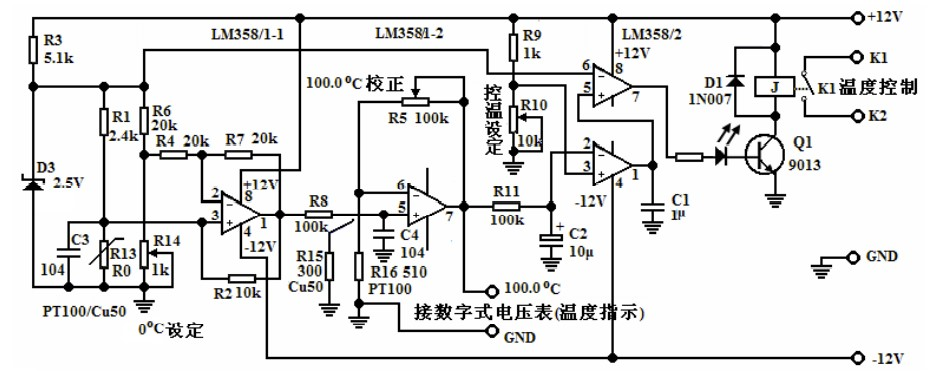
\includegraphics[width=0.8\textwidth]{img//1.jpg}
	\caption{基于PT100或(Cu50)温度传感器的温度控制仪电路图}
\end{figure}

(1) 温度显示

如图\ref*{fig:3},$R_t=R_0(1+A_t)$

当$t=100^{\circ}C$时,$A_{V1}=\frac{1+R_5}{R_16}$

当$U_{GND}=0$时,$A_{V1}=1+\frac{100}{R_0(1+373.5)}$

当温度升至$100^{\circ}C$时,$U=A_{V1}\times V_6$

故温度显示灵敏度为$100mV/^{circ}C$.

(2) 温度控制

设定温度控制在$80^{\circ}C$,有$V_3=3.5316V$。当温度低于控制温度时,$V_4\approx V_3 < V_5$,
$A_2 $,$A_3$,$Q_1$导通,发光LED点亮,继电器吸合,控制加温器开始工作。当温度达到设定的$80^{\circ}C$时,
$V_4> V_5$,$A_2 $, $A_3$ ,$Q_1$ 截止,发光LED熄灭,控制加热器停止工作。

2.基于LM35电压型温度传感器的数显温度控制仪

\begin{figure}[htbp]
	\centering
	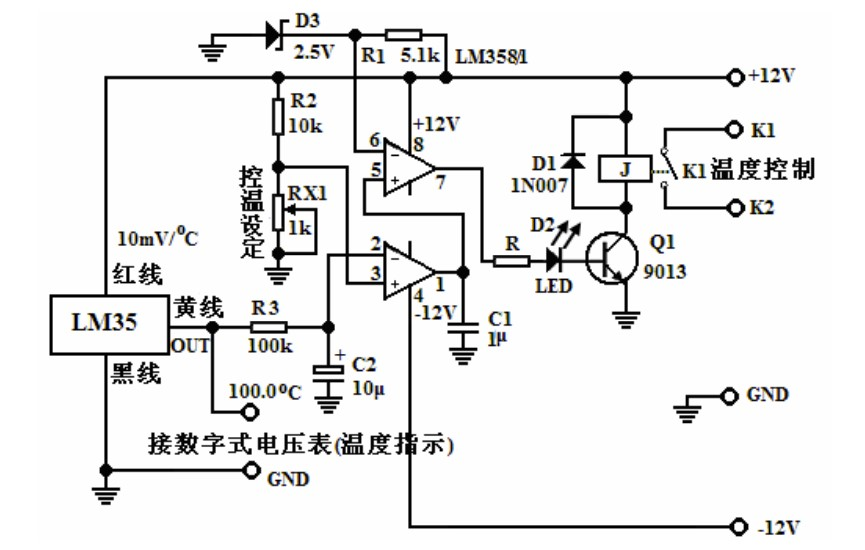
\includegraphics[width=0.8\textwidth]{img//2.jpg}
	\caption{基于LM35电压型温度传感器的数显温度控制仪电路图}
\end{figure}

(1) 温度显示

输出电压量程为1V,对应测温范围为$0-100^{\circ}C$,故温度显示灵敏度为$10mV/^{\circ}C$.

(2) 温度控制

设定温度控制在$80^{\circ}C$,有$V_3=3.5316V$。当温度低于控制温度时,$V_4\approx V_3 < V_5$,
$A_2 $,$A_3$,$Q_1$导通,发光LED点亮,继电器吸合,控制加温器开始工作。当温度达到设定的$80^{\circ}C$时,
$V_4> V_5$,$A_2 $, $A_3$ ,$Q_1$ 截止,发光LED熄灭,控制加热器停止工作。


\end{document}
